\documentclass[12pt,a4paper]{article}
\usepackage[UTF8]{ctex}
\usepackage{geometry}
\usepackage{graphicx}
\usepackage{float}
\usepackage{amsmath}
\usepackage{amsfonts}
\usepackage{amssymb}
\usepackage{booktabs}
\usepackage{multirow}
\usepackage{array}
\usepackage{longtable}
\usepackage{enumerate}
\usepackage{fancyhdr}
\usepackage{lastpage}
\usepackage{hyperref}
\usepackage[normalem]{ulem}

% 页面设置
\geometry{left=2.5cm,right=2.5cm,top=2.5cm,bottom=2.5cm}
\setlength{\headheight}{15pt}

% 页眉页脚设置
\pagestyle{fancy}
\fancyhf{}
\fancyhead[C]{实\hspace{0.5em}验\hspace{0.5em}原\hspace{0.5em}始\hspace{0.5em}记\hspace{0.5em}录}
\fancyfoot[L]{\parbox[t]{\textwidth}{实验人员：\underline{ 陈恪瑾}  学号：\underline{U202413925}  同组人员：\underline{黄伟峰}}}
\fancyfoot[R]{教师签字：\underline{\hspace{3cm}}}

\begin{document}

% 正文第一行标题
\noindent
{\Large \textbf{实验十：}\underline{\textbf{二阶电路的响应}}} \hfill {\Large \textbf{实验台编号：}\underline{\textbf{05}}}
\vspace{0.5cm}

\section*{一、实验注意事项}
\begin{enumerate}
    \item 实验前应设计好电路参数，而且注意电感内含有的$ 150 \Omega $电阻。
    
    \item 实验采样电阻$ r $应远小于回路阻抗。
    
\end{enumerate}

\section*{二、实验线路}
\begin{figure}[H]
    \centering
    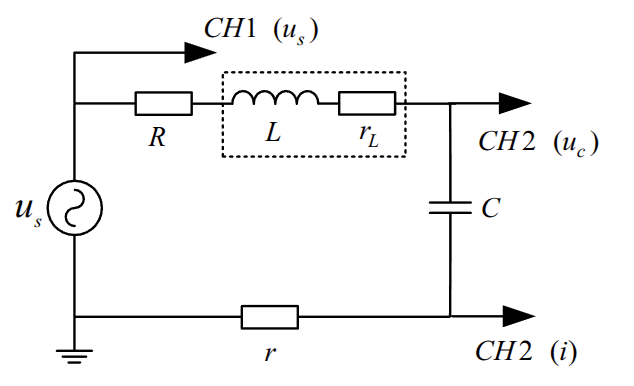
\includegraphics[width=0.8\textwidth]{E10_preview/schematic.png}
    \caption{RLC二阶串联电路}
    \label{fig:circuit}
\end{figure}

\section*{三、实验数据}
\begin{enumerate}
    \item 记录实验结果曲线
\end{enumerate}

\end{document}
